\chapter{Getting Started}\label{chap:2}
\label{ch:start}

This chapter explains how to install REGEN, how the main window is organized, how projects are opened and saved,
how to start from one of the built-in case studies or from existing data, and how results are exported.

\section{Installation}
\label{sec:ch02-install}

\subsection{Requirements}
REGEN runs on 64-bit Windows 10 and Windows 11. The installer contains everything that is needed (the program and
its libraries); Python or other software does not have to be installed. ANN training on several CPU cores starts one
worker process per core and therefore needs more memory than the other calculations (see
Section~\ref{sec:ch02-cores}).

\subsection{Installing}
\begin{enumerate}
  \item Download the installer \texttt{REGEN-Setup-7.0.0.exe} (the number is the version) from the
        \emph{Releases} page of the repository, \url{https://github.com/chumporium/REGEN/releases}.
  \item Start the installer. Because the installer is not code-signed,
        Windows SmartScreen may show the message ``Windows protected your PC''. Click \ui{More info}, check that the
        file name is the REGEN installer you downloaded, and click \ui{Run anyway}.
  \item The installer asks for the installation mode. Choose \ui{Install for me only} to install REGEN for your
        own Windows account; no administrator rights are needed and the program is installed in
        \texttt{\%LOCALAPPDATA\%\textbackslash Programs\textbackslash REGEN}. Choose \ui{Install for all users} to
        install it in \texttt{Program Files} for every account on the computer (administrator rights required).
  \item Select the additional tasks: \ui{Create a desktop shortcut} and \ui{Open .doe files with REGEN} (file
        association, so that double-clicking a project file in Explorer opens it in REGEN). Both are selected by
        default.
  \item Click \ui{Install}. At the end, REGEN can be started directly. A Start menu entry \ui{REGEN} is created.
\end{enumerate}

Installing a new version over an older one keeps your project files and the list of recent projects. The installer
also replaces earlier versions that were installed under the name DOE Studio (it removes their old shortcuts).

\subsection{Uninstalling}
Use \menupath{Start $\rightarrow$ REGEN $\rightarrow$ Uninstall REGEN}, or \menupath{Settings $\rightarrow$ Apps
$\rightarrow$ Installed apps $\rightarrow$ REGEN $\rightarrow$ Uninstall}. Uninstalling removes the program and the
file association but never your \texttt{.doe} project files or exported results.

\subsection{Self-test}
\label{sec:ch02-selftest}
The installed program contains a self-test that exercises the main computations (all design families, RSM, GLM,
split-plot REML, mixture and optimal designs, ANN training and architecture search, learning curve, NSGA-II and
NSGA-III, the ANN vs RSM comparison, sensitivity analysis, PDF and Excel export) without opening a window. It is
useful after installation on a new computer or when a result looks suspicious. Run it from a command prompt:
\begin{verbatim}
start /wait "" "C:\path\to\REGEN\REGEN.exe" --self-test C:\temp\regen_test
\end{verbatim}
(\texttt{start /wait} makes the command prompt wait until the test has finished.) The folder is created if
necessary. REGEN writes the file \texttt{selftest.log} there, together with the plots, PDF reports and Excel files
produced during the test. A successful test ends with the line \texttt{SELFTEST OK}; if something fails, the log
contains the error message, which is useful when reporting a problem. The test can take several minutes.

\section{The main window}
\label{sec:ch02-window}

\begin{figure}[htbp]
\centering
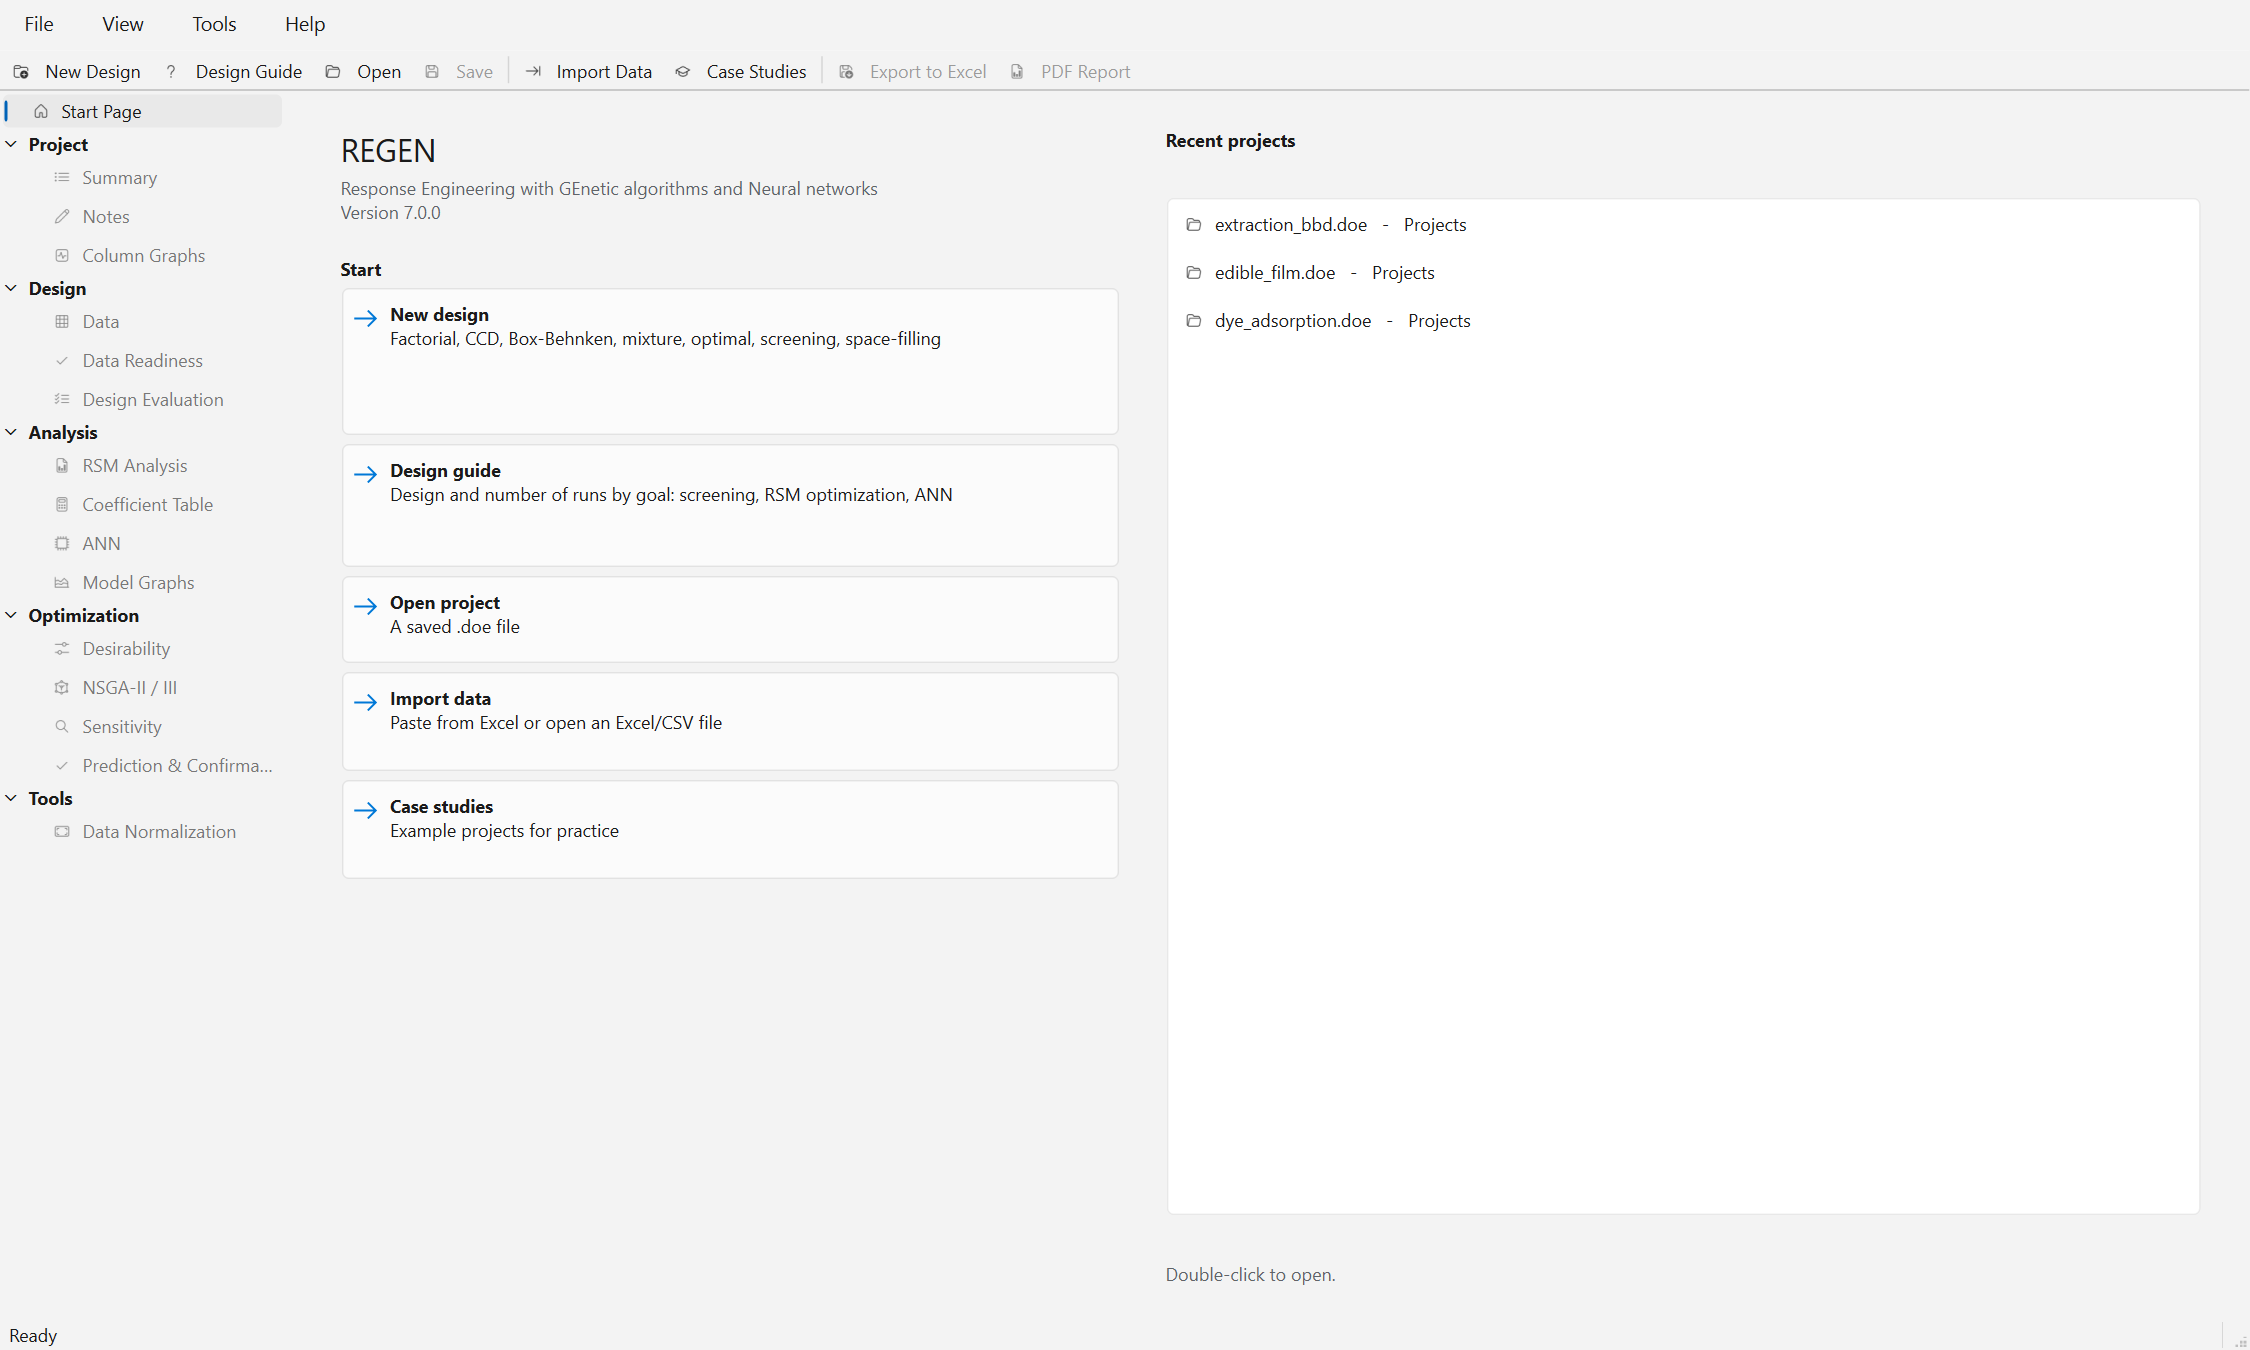
\includegraphics[width=0.85\linewidth]{start_page.png}
\caption{The main window with the Start Page. Left: navigation tree with the pages grouped by work stage. Center:
the five start buttons. Right: recent projects. Save, Export to Excel and PDF Report are greyed out because no
project is open.}
\label{fig:ch02-start}
\end{figure}

The main window (Figure~\ref{fig:ch02-start}) has a menu bar, a toolbar, the navigation tree on the left, the work
page on the right and a status bar at the bottom. The divider between the tree and the page can be dragged.

\subsection{Start Page}
The Start Page is shown when REGEN starts. Its five buttons are shortcuts to the most common first steps:
\begin{description}
  \item[\ui{New design}] ``Factorial, CCD, Box-Behnken, mixture, optimal, screening, space-filling'': opens the
        New Design dialog (Chapter~\ref{chap:3}).
  \item[\ui{Design guide}] ``Design and number of runs by goal: screening, RSM optimization, ANN'': opens the
        Design Guide (Chapter~\ref{chap:3}).
  \item[\ui{Open project}] ``A saved .doe file''.
  \item[\ui{Import data}] ``Paste from Excel or open an Excel/CSV file'' (Section~\ref{sec:ch02-import}).
  \item[\ui{Case studies}] ``Example projects for practice'' (Section~\ref{sec:ch02-cases}).
\end{description}
The list \ui{Recent projects} on the right shows the last projects that were opened or saved and still exist, as
``file name - folder''; hovering shows the full path. Double-click an entry to open it.

\subsection{Navigation tree}
\label{sec:ch02-tree}
The pages are grouped by work stage (Table~\ref{tab:ch02-pages}). All pages except the Start Page need an open
project; they are greyed out until a project is opened or created. Clicking a page refreshes it with the current
project state, so a page always shows the current models and data. The same pages can be reached from the
\ui{View} menu.

\begin{table}[htbp]
\centering
\caption{Pages of the navigation tree.}
\label{tab:ch02-pages}
\small
\begin{tabularx}{\linewidth}{@{}llX@{}}
\toprule
Group & Page & Purpose \\
\midrule
 & Start Page & Start buttons and recent projects \\
Project & Summary & Factors, responses, models and other project contents at a glance \\
 & Notes & Free-text notes (saved in the project and printed in the PDF report) \\
 & Column Graphs & Scatter plots, histograms, box plots and correlations of the raw data columns \\
Design & Data & The data sheet: runs, factor settings and responses (page title ``Data \& Design'') \\
 & Data Readiness & Scores for modeling and optimization, recommendations, suggested runs \\
 & Design Evaluation & Degrees of freedom, power, aliasing, VIF, efficiencies, FDS \\
Analysis & RSM Analysis & Model selection, ANOVA, equations, diagnostics, Box-Cox, effects, GLM, REML \\
 & Coefficient Table & Coded coefficients of all responses side by side \\
 & ANN & Artificial neural networks, architecture search, learning curve \\
 & Model Graphs & Contour, surface, effect, interaction, overlay, desirability, POE and mixture plots \\
Optimization & Desirability & Desirability optimization (page title ``Desirability Optimization'') \\
 & NSGA-II / III & Multi-objective optimization, Pareto front, checks C and D \\
 & Sensitivity & Parametric study and sensitivity analysis \\
 & Prediction \& Confirmation & Prediction, CI/PI and confirmation runs \\
Tools & Data Normalization & View and export normalized data \\
\bottomrule
\end{tabularx}
\end{table}

\subsection{Menus}
\label{sec:ch02-menus}
Table~\ref{tab:ch02-menus} lists every menu item. Items that need a project (\ui{Save}, \ui{Save As\dots},
\ui{Export to Excel\dots}, \ui{PDF Report\dots} and the pages) are disabled while no project is open.

\begin{table}[htbp]
\centering
\caption{Menu items. Shortcuts are listed in Appendix~A.}
\label{tab:ch02-menus}
\small
\begin{tabularx}{\linewidth}{@{}llX@{}}
\toprule
Menu & Item & Action \\
\midrule
File & \ui{New Design\dots} (Ctrl+N) & Create a new design (Chapter~\ref{chap:3}) \\
 & \ui{Design Guide\dots} & Choose a design and run count by goal; \ui{Create This Design\dots} fills in New
   Design \\
 & \ui{Open\dots} (Ctrl+O) & Open a project file (\texttt{*.doe}) \\
 & \ui{Open Recent} & Submenu with the recent projects (up to 8) \\
 & \ui{Import Data\dots} & Create a project from existing data (Section~\ref{sec:ch02-import}) \\
 & \ui{Case Studies\dots} & Open a built-in example (Section~\ref{sec:ch02-cases}) \\
 & \ui{Save} (Ctrl+S) & Save the project; asks for a file name the first time \\
 & \ui{Save As\dots} (Ctrl+Shift+S) & Save under a new name (\texttt{.doe} is added if missing) \\
 & \ui{Export to Excel\dots} & Data and RSM results as an Excel workbook (Section~\ref{sec:ch02-excel}) \\
 & \ui{PDF Report\dots} & Complete report as PDF (Section~\ref{sec:ch02-pdf}) \\
 & \ui{Exit} (Alt+F4) & Close REGEN (asks to save unsaved changes) \\
\addlinespace
View & one item per page & Same pages as the navigation tree, separated by group \\
\addlinespace
Tools & \ui{Data Normalization} & Opens the Data Normalization page \\
\addlinespace
Help & \ui{User Manual} (F1) & Opens this manual (PDF) \\
 & \ui{Getting Started} & Short summary of the workflow in six steps \\
 & \ui{Design Guide (RSM / ANN Run Counts)\dots} & Same as File $\rightarrow$ Design Guide \\
 & \ui{About REGEN} & Version, authors and license \\
\bottomrule
\end{tabularx}
\end{table}

Before \ui{New Design\dots}, \ui{Design Guide\dots} (when a design is created from it), \ui{Open\dots}, a recent
project, \ui{Import Data\dots}, \ui{Case Studies\dots} and when the window is closed, REGEN checks for unsaved
changes and asks ``The current project has unsaved changes. Save it first?'' with the buttons \ui{Save},
\ui{Discard} and \ui{Cancel}. If an ANN search or an NSGA run is still running when the window is closed, it is
stopped first; a running sensitivity calculation is allowed to finish.

\subsection{Toolbar}
The toolbar repeats the most used file commands: \ui{New Design}, \ui{Design Guide}, \ui{Open}, \ui{Save} $|$
\ui{Import Data}, \ui{Case Studies} $|$ \ui{Export to Excel}, \ui{PDF Report}.

\subsection{Title bar and status bar}
The window title shows the project file name followed by ``- REGEN''; ``Untitled'' is used for a project that has
not been saved yet, and an asterisk after the name means that there are unsaved changes. The right part of the
status bar shows the design description, the number of runs and the number of complete runs (runs whose responses
are all filled in), for example
\begin{quote}\small
\texttt{Box-Behnken Design (BBD) - 3 factors, 17 runs \ \ |\ \ 17 runs, 17 complete}
\end{quote}
and, if runs are excluded from the analysis, ``, $m$ excluded''. Short messages such as ``Saved: \dots'' or
``Exported to \dots'' appear on the left for a few seconds.

\section{Project files}
\label{sec:ch02-files}

A project is saved as one file with the extension \texttt{.doe} (filter ``REGEN Project (*.doe)''). The file is
plain UTF-8 text in JSON format (Appendix~A describes its structure) and contains:
\begin{itemize}
  \item the design: design type and options (including the random seed), factors with their ranges, levels and
        standard deviations, mixture total, linear constraints, blocks, whole plots and hard-to-change factors;
  \item the runs: coded factor settings, point types, run order, all response values, and the list of runs excluded
        from the analysis;
  \item the responses with their names, units, type (normal, binomial, Poisson) and number of trials;
  \item the model settings of each response (model order, selected terms, transformation) and the choice RSM or
        ANN for each response;
  \item the trained ANN models (weights, normalization and the cross-validated diagnosis), so that they do not
        have to be trained again;
  \item the optimization criteria of the Desirability page and the notes;
  \item the results of the last analyses: architecture-search results, learning curves, desirability solutions,
        the last NSGA-II/III result and the ANN vs RSM front comparison. A single result that would be very large
        (more than 5 million characters) is not saved; the project still opens without it.
\end{itemize}
RSM models are not stored as numbers but refitted from the data and the model settings when the project is opened,
so they always match the data. The sensitivity results and the confirmation values typed on the Prediction page are
not saved; they are quick to recompute.

Project files of the earlier versions named DOE Studio (versions 1 to 6) open without conversion, including older
point-type labels, and the recent-project list of those versions is kept. Files written before results were saved
simply open without stored results.

A \texttt{.doe} file can be opened by \menupath{File $\rightarrow$ Open\dots}, from \ui{Open Recent}, from the
Start Page, or by double-clicking it in Explorer when the file association was selected during installation. After
opening, the Data page is shown.

\section{Case studies}
\label{sec:ch02-cases}

\begin{figure}[htbp]
\centering
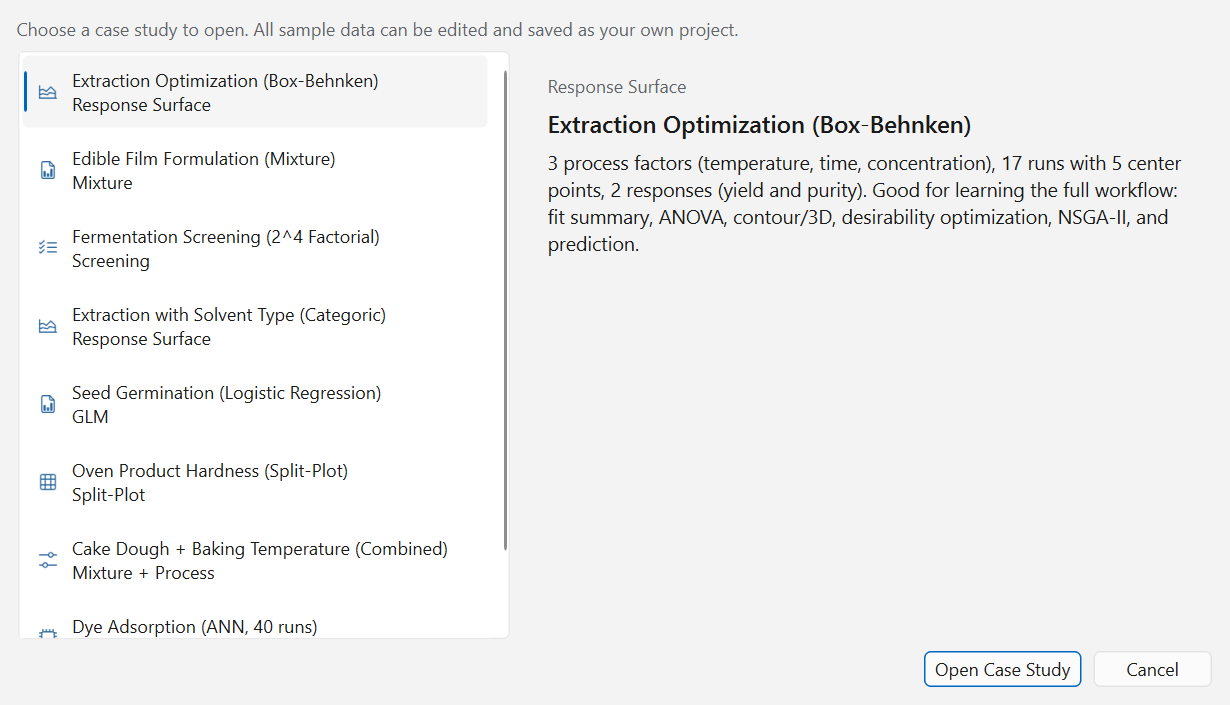
\includegraphics[width=0.65\linewidth]{case_studies.png}
\caption{The Case Studies dialog with the first case selected.}
\label{fig:ch02-cases}
\end{figure}

The eight built-in case studies (\menupath{File $\rightarrow$ Case Studies\dots}, Figure~\ref{fig:ch02-cases})
cover every analysis family of REGEN. Select a case in the list to see its description, then click \ui{Open Case
Study} (or double-click). The project opens on the Data page as an untitled project; it can be edited and saved as
your own project. The data are simulated from known equations with Gaussian noise and fixed random seeds, so every
user sees exactly the same numbers, and the ``true'' behavior is known, which makes the cases suitable for learning
and for checking the methods. Table~\ref{tab:ch02-cases} lists the cases.

\begin{table}[htbp]
\centering
\caption{Built-in case studies (in the order of the dialog).}
\label{tab:ch02-cases}
\scriptsize
\begin{tabularx}{\linewidth}{@{}p{0.17\linewidth}p{0.18\linewidth}p{0.22\linewidth}p{0.12\linewidth}X@{}}
\toprule
Case (category) & Design & Factors (range) & Responses & Good for learning \\
\midrule
Extraction Optimization (Box-Behnken) (Response Surface) &
Box-Behnken, 3 factors, 5 center points, 17 runs &
Temperature 60--80 \textdegree C; Time 30--90 min; Concentration 1--3 \% &
Yield (\%), Purity (\%) &
The whole workflow: fit summary, ANOVA, diagnostics, graphs, desirability, NSGA-II, sensitivity, prediction;
ANN vs RSM with few runs \\
\addlinespace
Edible Film Formulation (Mixture) (Mixture) &
Simplex lattice \{3,\,2\} with axial points and replicated vertices and centroid, total 100, 14 runs &
Starch $\ge$ 50 \%; Glycerol $\ge$ 10 \%; Chitosan $\ge$ 10 \% (each up to its lower limit + 30) &
Tensile Strength (MPa), Elongation (\%) &
Pseudo-components, Scheff\'e models, ternary contour, trace plot \\
\addlinespace
Fermentation Screening ($2^4$ Factorial) (Screening) &
Unreplicated two-level full factorial, 16 runs &
Temperature 30--50 \textdegree C; pH 5--7; Agitation 100--200 rpm; Inoculum 2--6 \% &
Biomass (g/L) &
Half-normal and Pareto plots of effects, Lenth's method \\
\addlinespace
Extraction with Solvent Type (Categoric) (Response Surface) &
Rotatable CCD in 2 factors with 3 center points, crossed with 3 solvents, 33 runs &
Temperature 40--60 \textdegree C; Time 2--6 h; Solvent (Ethanol, Methanol, Acetone) &
Yield (\%) &
Categoric factors, effect coding, one equation per level, optimization across levels \\
\addlinespace
Seed Germination (Logistic Regression) (GLM) &
Rotatable CCD, 2 factors, 5 center points, 13 runs &
Temperature 20--35 \textdegree C; Humidity 60--90 \% &
Germinated (seeds out of 50 per run) &
Binomial response, logistic regression, likelihood-ratio tests, odds ratios \\
\addlinespace
Oven Product Hardness (Split-Plot) (Split-Plot) &
Two-level full factorial, 2 replicates, oven temperature hard to change, 4 whole plots, 16 runs &
Oven Temperature 150--190 \textdegree C; Time 10--20 min; Concentration 1--3 \% (factor standard deviations
given) &
Hardness (N) &
Split-plot REML, variance components, whole-plot tests, propagation of error \\
\addlinespace
Cake Dough + Baking Temperature (Combined) (Mixture + Process) &
I-optimal combined design, model Quadratic $\times$ Linear, total 100, 22 runs (12 model, 5 lack of fit, 5
replicates) &
Flour 50--80 \%; Sugar 10--30 \%; Fat 10--30 \%; Temperature 160--200 \textdegree C (process) &
Texture (score) &
Combined mixture-process models, constrained mixture region \\
\addlinespace
Dye Adsorption (ANN, 40 runs) (Machine Learning) &
Historical data, 40 runs (Latin hypercube) &
pH 2--10; Adsorbent Dose 0.5--4 g/L; Contact Time 10--120 min; Initial Concentration 20--200 mg/L &
Removal Efficiency (\%) &
Strongly nonlinear data: data readiness, ANN adequacy, architecture search, learning curve, normalization, RSM vs
ANN \\
\bottomrule
\end{tabularx}
\end{table}

\section{Importing existing data}
\label{sec:ch02-import}

\paragraph{Purpose.} \ui{Import Data\dots} creates a project from data that already exist: results from earlier
experiments, plant records, a table in Excel or CSV, or a design made in another DOE program. The imported runs
become a historical-data project that can be analyzed like a designed experiment.

\begin{figure}[htbp]
\centering
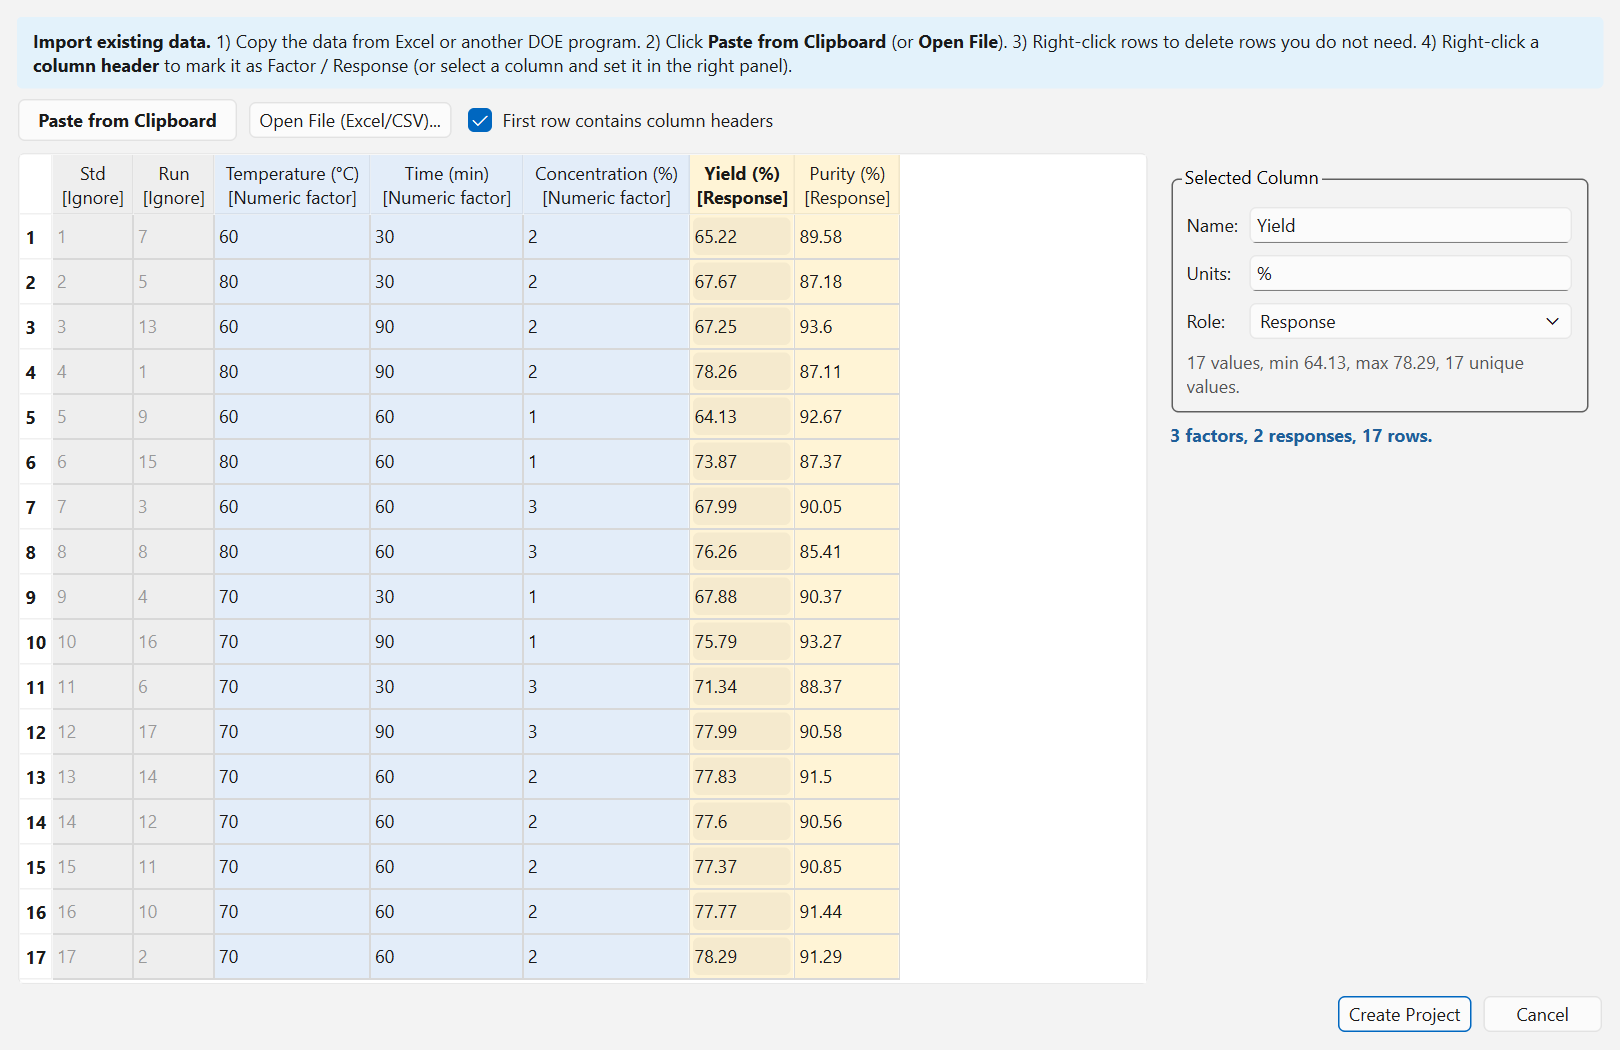
\includegraphics[width=0.8\linewidth]{import_dialog.png}
\caption{The Import Data Set dialog after pasting the 17-run Box-Behnken table. Std and Run are recognized as
bookkeeping columns (Ignore), the three factor columns as numeric factors and the two columns marked R1/R2 as
responses; names and units are taken from the headers.}
\label{fig:ch02-import}
\end{figure}

\paragraph{How to use.}
\begin{enumerate}
  \item Copy the table (with a header row if possible) in Excel or another program, then choose
        \menupath{File $\rightarrow$ Import Data\dots} and click \ui{Paste from Clipboard}. Alternatively click
        \ui{Open File (Excel/CSV)\dots} and select an \texttt{.xlsx}, \texttt{.xlsm}, \texttt{.csv} or
        \texttt{.txt} file.
  \item Check \ui{First row contains column headers}. It is set automatically when the first row contains text
        and there is more than one row.
  \item Check the role of every column. The role is shown below the column name in the header and by the column
        color. To change it, right-click the column header and choose a role, or click a column and set
        \ui{Name}, \ui{Units} and \ui{Role} in the panel \ui{Selected Column} on the right. The panel also shows the
        number of values, the minimum, maximum and number of unique values (or the levels of a categoric column).
  \item Delete rows that should not be imported: select cells in those rows, right-click and choose
        \ui{Delete $n$ Selected Rows}.
  \item For mixture data, set \ui{Mixture total} (see below).
  \item Click \ui{Create Project}. The project opens on the RSM Analysis page and is marked as unsaved.
\end{enumerate}

\paragraph{Column roles.} Table~\ref{tab:ch02-roles} lists the roles. REGEN proposes a role for every column:
\begin{itemize}
  \item a column whose header is a bookkeeping name (Std, Run, No, No., Number, Order, ID, Block, \#, and the
        Indonesian equivalents) or that is empty becomes \ui{Ignore};
  \item a column with at least 80\,\% numeric cells becomes \ui{Numeric factor}, otherwise \ui{Categoric factor};
  \item a header that starts with ``R1:'', ``R2:'', \dots{} (the style used by DOE programs) marks a
        \ui{Response}; if no column is a response, the last numeric column becomes the response.
\end{itemize}
Header prefixes ``A:'' or ``R1:'' are removed, and a unit written in parentheses or square brackets at the end of the
header (``Temperature (\textdegree C)'', ``Yield [\%]'') is moved to the \ui{Units} field. Cells that are not numbers
in a numeric, component or response column are shown in red.

\begin{table}[htbp]
\centering
\caption{Column roles in the Import Data Set dialog.}
\label{tab:ch02-roles}
\small
\begin{tabularx}{\linewidth}{@{}lX@{}}
\toprule
Role & Meaning \\
\midrule
\ui{Numeric factor} & Continuous factor. Its range (low, high) is set to the minimum and maximum of the data. \\
\ui{Categoric factor} & Factor with named levels (2 to 20 levels), in the order of first appearance. \\
\ui{Mixture component} & Component of a mixture; lower limit = data minimum, upper limit = data maximum. All
  factors must then be components (at least 2). \\
\ui{Response} & Measured response (empty cells are allowed and stay empty). \\
\ui{Ignore} & Not imported (run numbers, standard order, block labels, comments). \\
\bottomrule
\end{tabularx}
\end{table}

\paragraph{Separators and decimal marks.} Pasted Excel data are tab-separated. In text and CSV files the separator
is a semicolon when the first lines contain at least as many semicolons as commas, otherwise a comma. Numbers may use
a decimal point or a decimal comma; when both appear (``1.234,5'' or ``1,234.5'') the separator that comes last is
taken as the decimal mark. A number with only a comma, such as ``1,234'', is read as 1.234, so thousands separators
must not be used. From Excel workbooks the first worksheet is read, with the values (not the formulas) of the cells.
Completely empty rows and columns are dropped.

\paragraph{Mixture data.} When columns are marked as components, the group \ui{Mixture} appears with
\ui{Mixture total}, set automatically to the median of the row sums. If some rows do not add up to the total, REGEN
asks whether to continue (those rows are still analyzed). Mixture components cannot be combined with process
factors in an import.

\paragraph{Messages.} \ui{Create Project} checks the table and stops with a message if something is wrong, for
example ``Mark at least one Factor column and one Response column.'', ``Factor X is constant / empty - mark it as
Ignore.'', ``Column X, row 5 is not a number: 'n/a'.'' or ``X has 35 levels - should this column be numeric or
ignored?''. Chapter~\ref{chap:12} lists these messages with their remedies.

\paragraph{Result.} The design type is ``Historical Data (Process)'' or ``Historical Data (Mixture)''; the run
order is the row order and the point type of every run is ``Historical''. Factor cells of a historical project can
be edited on the Data page, and rows can be added or deleted there (Chapter~\ref{chap:4}).

\section{Exporting results}
\label{sec:ch02-export}

Every result of REGEN can leave the program, either as a complete report, as an Excel workbook, or table by table
and plot by plot.

\subsection{Export to Excel}
\label{sec:ch02-excel}
\menupath{File $\rightarrow$ Export to Excel\dots} writes a workbook (default name: the project name with
\texttt{.xlsx}):
\begin{itemize}
  \item sheet \texttt{Design}: the design description, then one row per run in run order with Std, Run, Block
        (if any), Type, Excluded (if runs are excluded), the factor settings in actual units (categoric factors as
        level names) and the responses;
  \item one sheet per response that has an RSM model (for example \texttt{R1 Yield}): transformation, ANOVA table
        (sum of squares, df, mean square, F-value, p-value), fit statistics (Std.\ Dev., Mean, C.V.\ \%, R$^2$,
        adjusted and predicted R$^2$, PRESS, Adeq Precision), coefficients in coded units (or pseudo-components)
        with standard errors, and the coefficients in actual units (one block per combination of categoric
        levels; for mixtures only when all lower limits are 0).
\end{itemize}
ANN models, optimization and sensitivity results are exported from their own pages (see below).

\subsection{PDF report}
\label{sec:ch02-pdf}
\menupath{File $\rightarrow$ PDF Report\dots} writes an A4 report and opens it. It contains, in this order:
\begin{enumerate}
  \item title, file name, date and the project notes;
  \item design summary: description, random seed, factor table, constraints and the data sheet (the first 200
        runs; the complete data are in the Excel export), with excluded runs marked;
  \item for each response: model and transformation, Fit Summary, ANOVA (or the GLM or split-plot tables), model
        equations, a diagnostics figure and a model graph;
  \item the Coefficient Table (when there is more than one response);
  \item for each response with an ANN: data adequacy, network summary and diagnosis, regression plots, RSM vs ANN,
        factor importance, network diagram and weights; learning curves if computed;
  \item Data Readiness and recommendations for each response;
  \item desirability optimization (criteria and the best solutions), if run;
  \item the NSGA-II/NSGA-III result (settings, objectives, convergence notes, Pareto front, convergence plot and the
        ten solutions with the highest TOPSIS score) and the ANN vs RSM comparison, if run.
\end{enumerate}
Results that are saved with the project (Section~\ref{sec:ch02-files}) are included also after the project is
reopened.

\subsection{Copying and exporting tables and plots}
\label{sec:ch02-copyexport}

\begin{figure}[htbp]
\centering

\includegraphics[width=\linewidth]{plot_toolbar.png}
\caption{The toolbar above every plot: Home, Back, Forward, Pan, Zoom, Subplot settings, Edit axes and Save image,
followed by \ui{Copy data} and \ui{Export data}.}
\label{fig:ch02-plottoolbar}
\end{figure}

\paragraph{Plots.} Every plot has a toolbar (Figure~\ref{fig:ch02-plottoolbar}). The first buttons reset the view,
step back and forward through zoom levels, pan, zoom to a rectangle, adjust the margins, edit axis limits, labels and
line styles, and save the image (PNG, SVG, PDF and other formats). The last two buttons export the \emph{data behind
the plot}:
\begin{description}
  \item[\ui{Copy data}] copies the data of every panel and series to the clipboard as a tab-separated table that
        can be pasted into Excel (title row, header row, values, blank row for each series);
  \item[\ui{Export data\dots}] saves the same data as an Excel workbook (one sheet per series, with the title in
        the first row and the column headers in the second) or as a CSV file (series below each other).
\end{description}
The same two commands are in the right-click menu of the plot, as \ui{Copy plot data} and \ui{Export plot
data\dots} (Figure~\ref{fig:ch02-plotmenu}); while Pan or Zoom is active the right mouse button belongs to that
tool. Lines, points, bars, histograms, error bars and heat maps are exported as drawn, with their legend names.
Contour, 3D surface, overlay, desirability and propagation-of-error plots export the full grid in actual units
with the plotted value at every grid point, and confidence bands and box plots export their underlying values, so a
plot can be redrawn exactly in another program.

\begin{figure}[htbp]
\centering
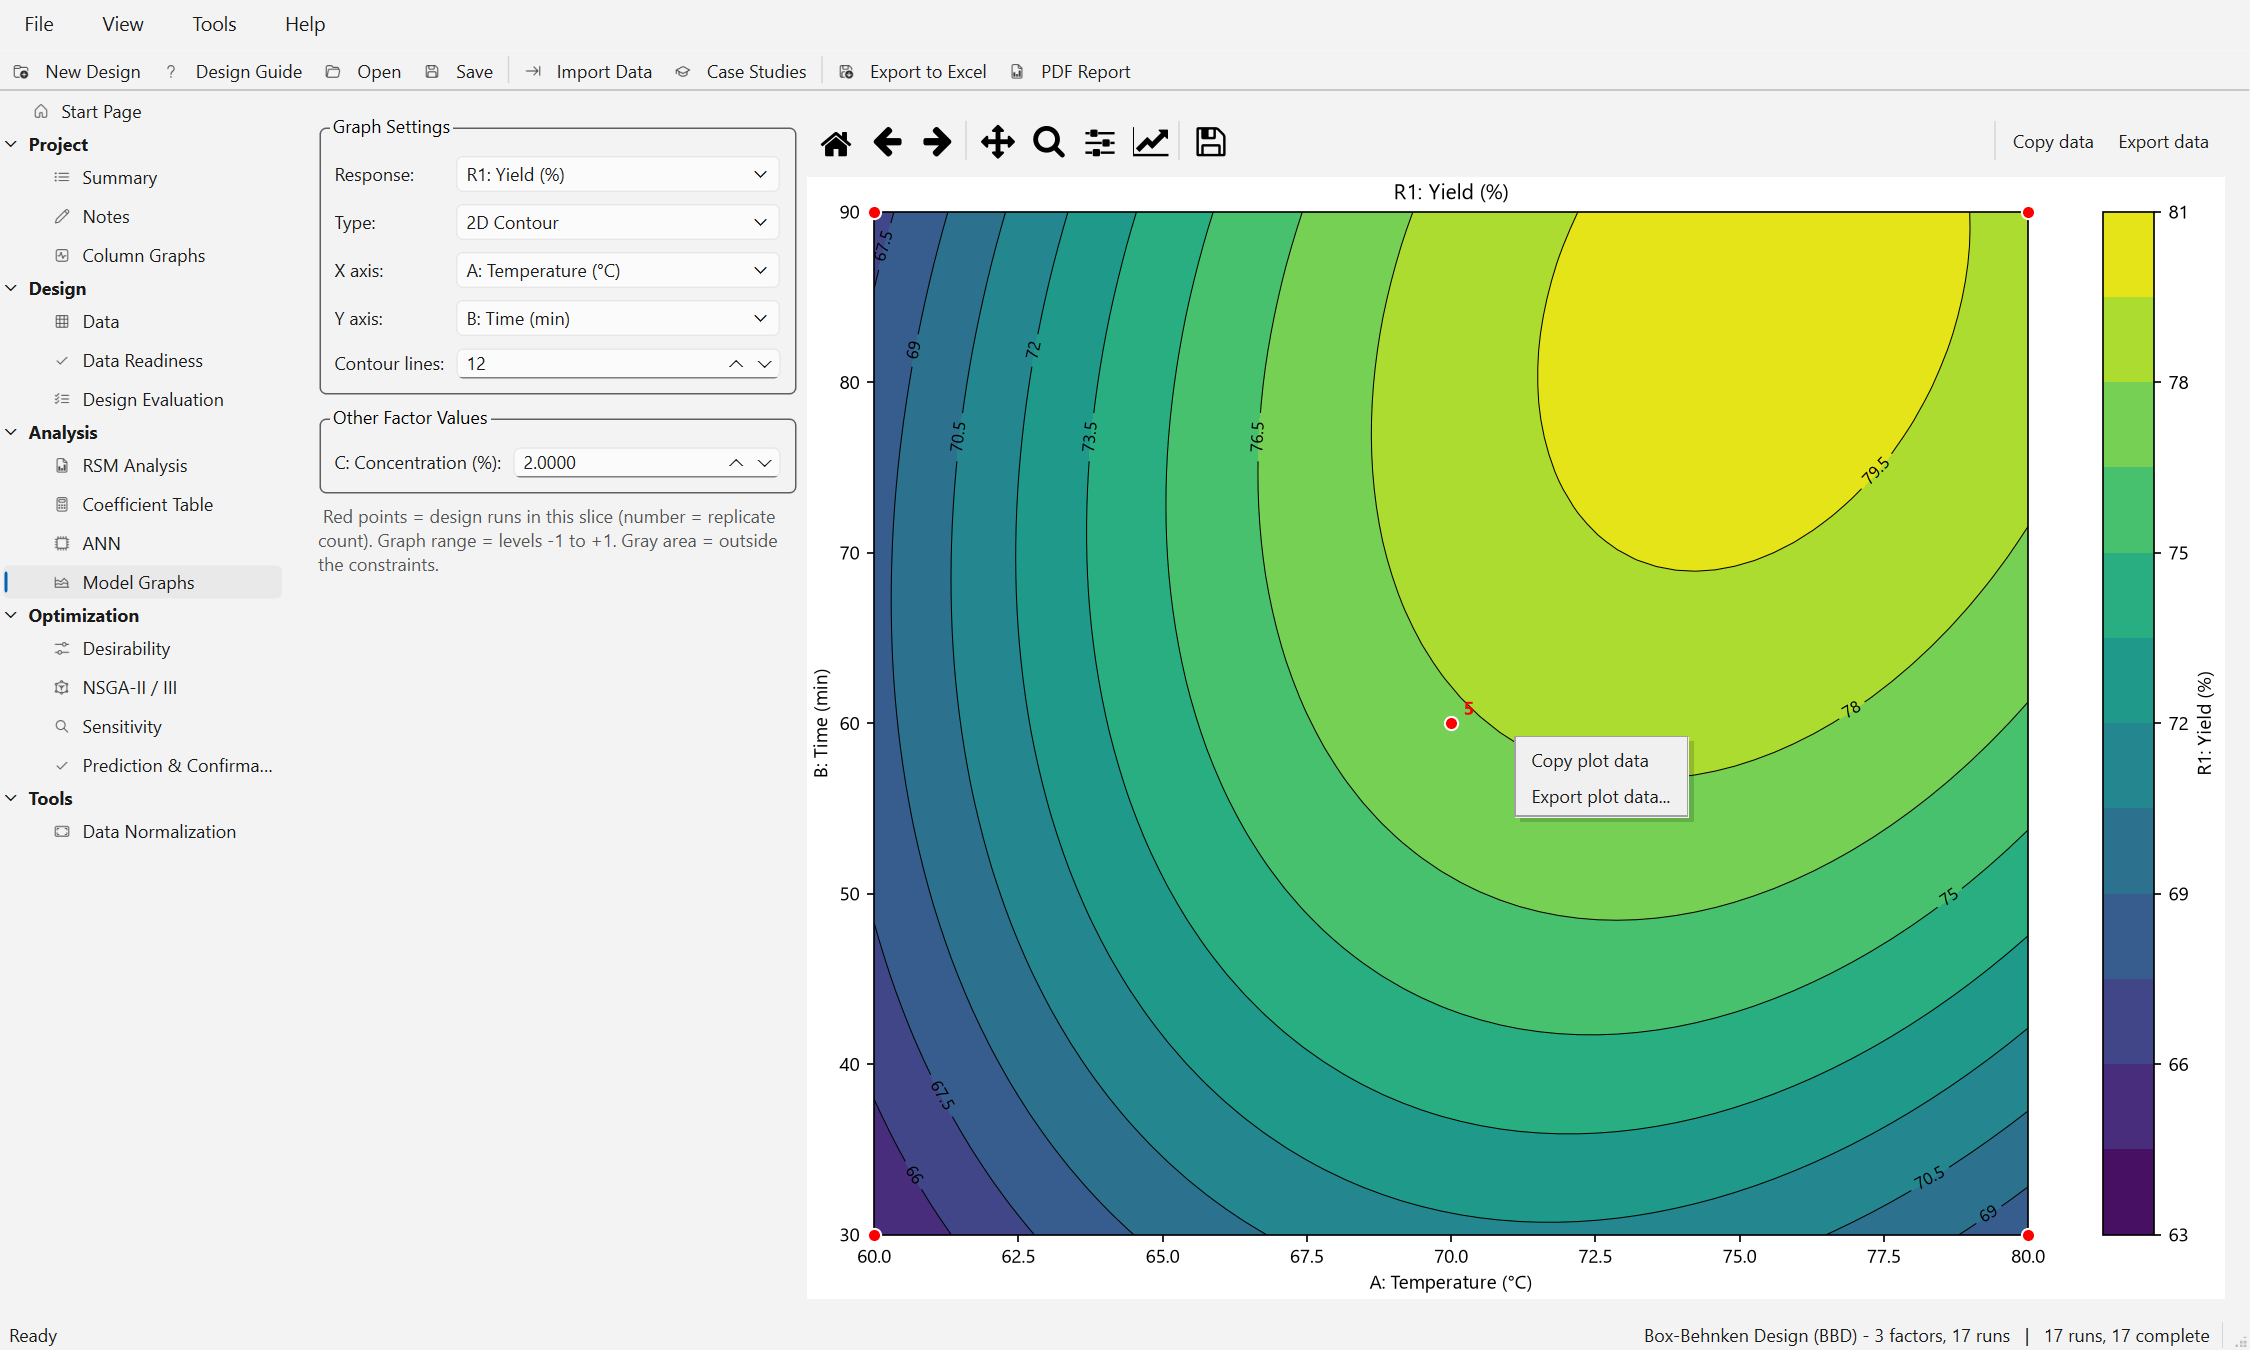
\includegraphics[width=0.5\linewidth]{plot_context_menu.png}
\caption{Right-click menu of a plot (here a contour plot).}
\label{fig:ch02-plotmenu}
\end{figure}

\paragraph{Result tables.} Every result table (solutions, Pareto solutions, diagnostics, normalized data, and so on)
has a right-click menu (Figure~\ref{fig:ch02-tablemenu}): \ui{Copy selected cells}, \ui{Copy selected cells with
column headers}, \ui{Copy entire table (for Excel)}, \ui{Copy entire table - decimal ','} (or \ui{'.'}: the
separator that is \emph{not} the Windows setting, useful when the data go to a computer with other regional
settings) and \ui{Export table\dots} (Excel or CSV; numeric cells are written as numbers). Ctrl+C copies the
selected cells.

\begin{figure}[htbp]
\centering
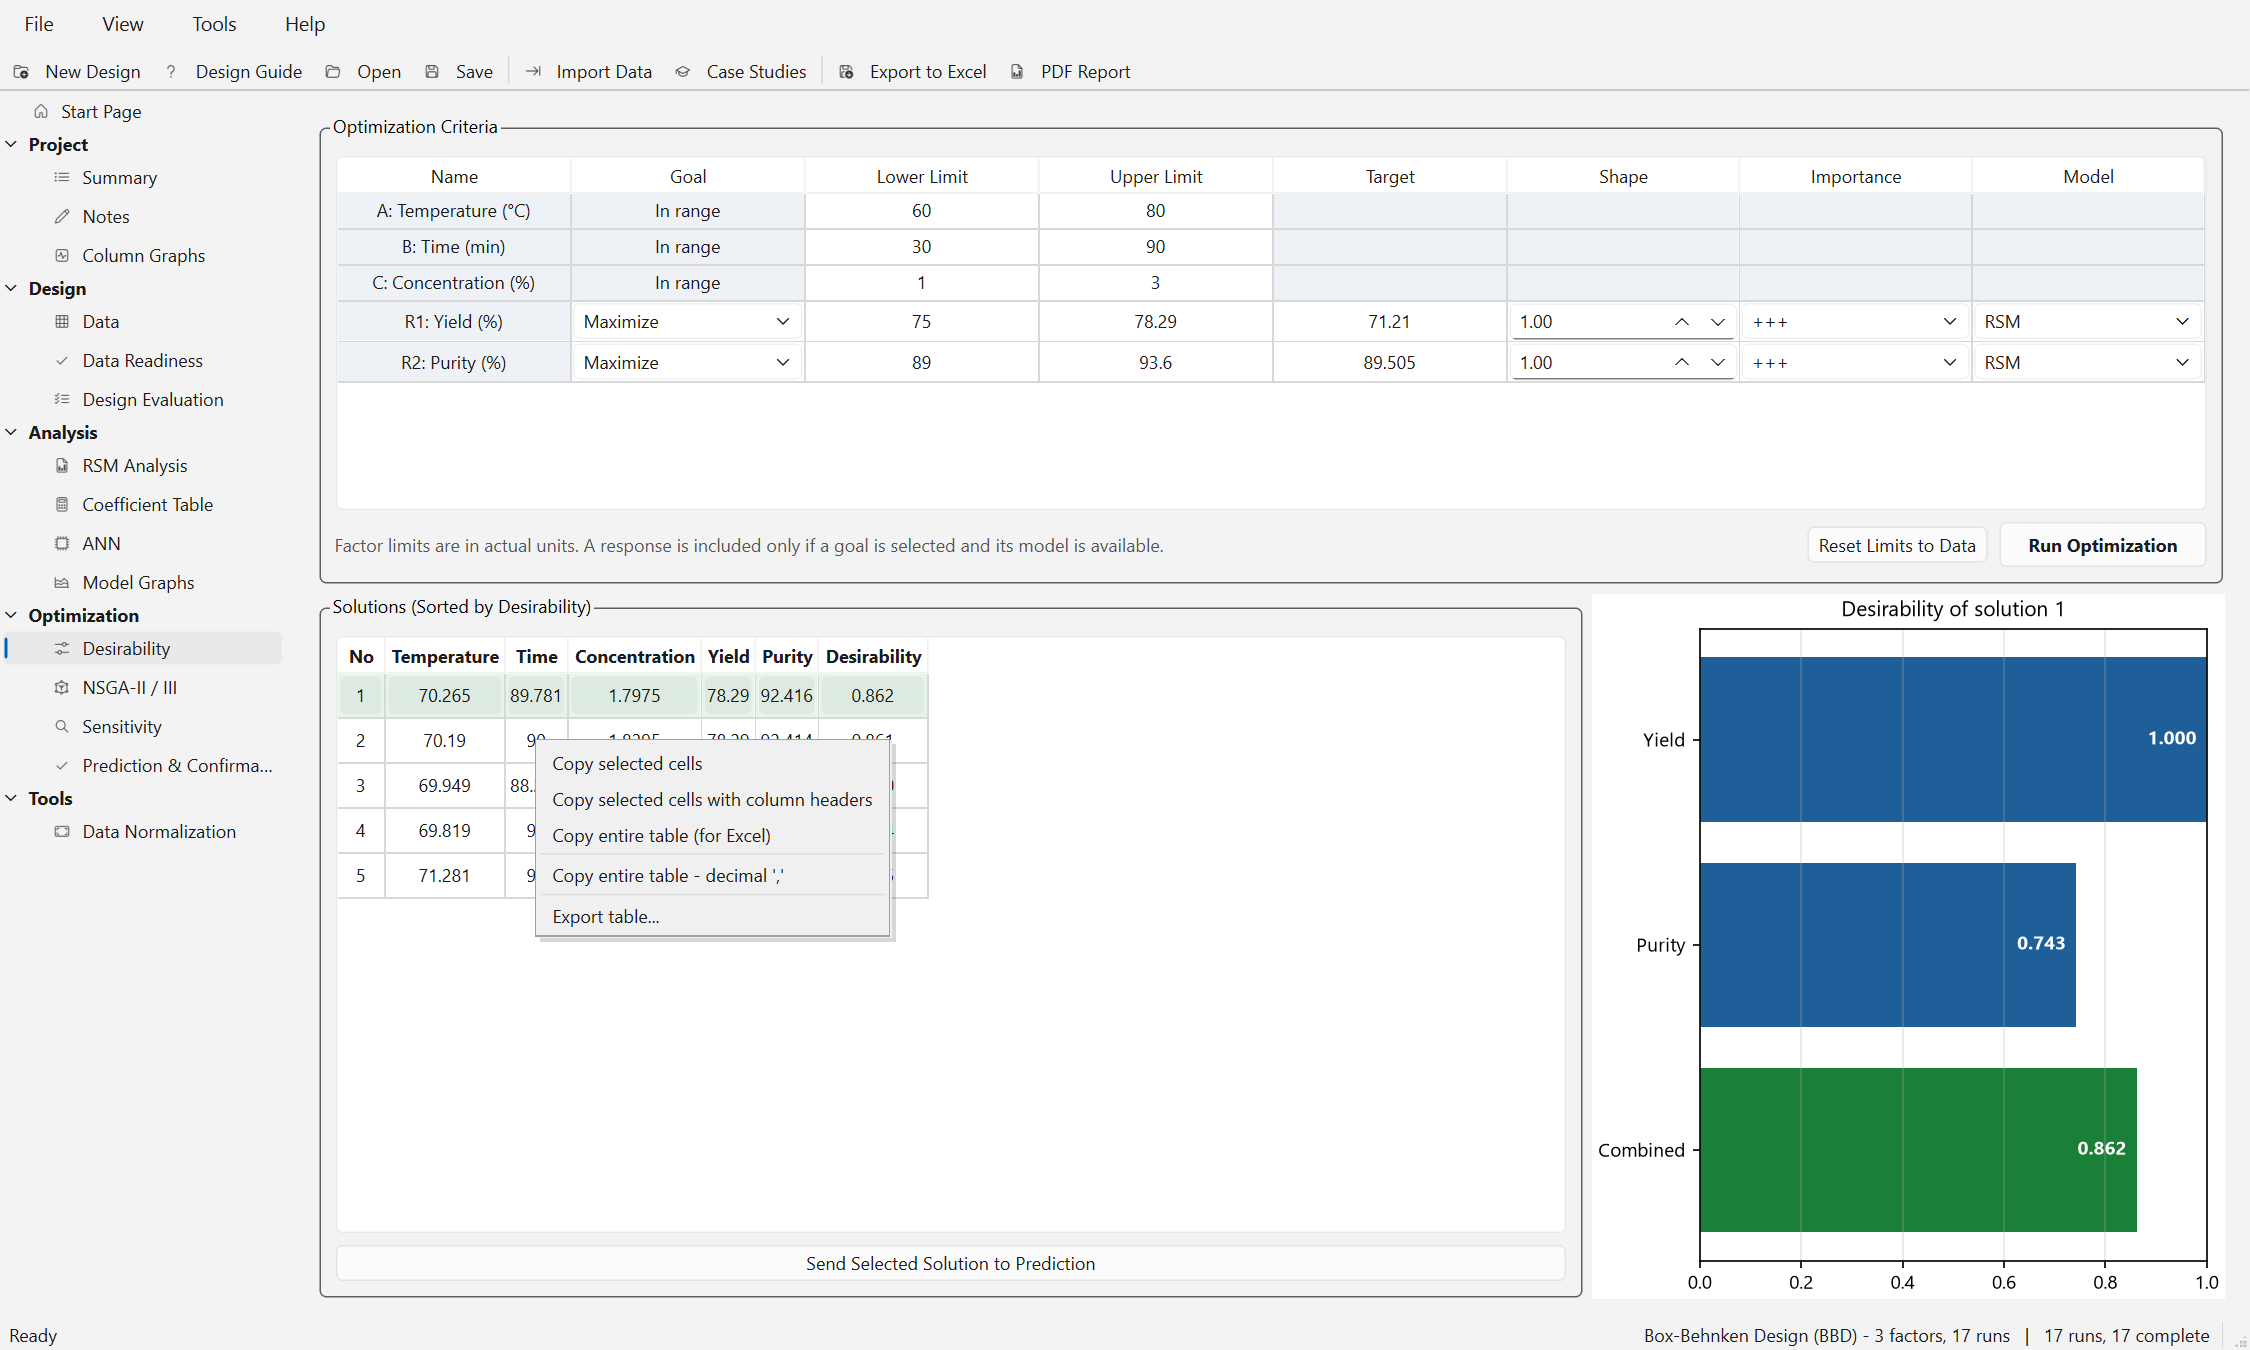
\includegraphics[width=0.5\linewidth]{table_context_menu.png}
\caption{Right-click menu of a result table (Desirability solutions).}
\label{fig:ch02-tablemenu}
\end{figure}

\paragraph{Report panels.} Text reports with tables (ANOVA, Fit Summary, Design Evaluation, Data Readiness, ANN
summary, NSGA convergence, sensitivity tables and others) have a right-click menu with the standard \ui{Copy} and
\ui{Select All} plus \ui{Copy all tables (for Excel)}, \ui{Copy all tables - decimal ','} and \ui{Export all
tables\dots}, which writes every table of the panel to its own sheet of an Excel workbook (or below each other in a
CSV file), named after the heading above the table (Figure~\ref{fig:ch02-reportmenu}).

\begin{figure}[htbp]
\centering
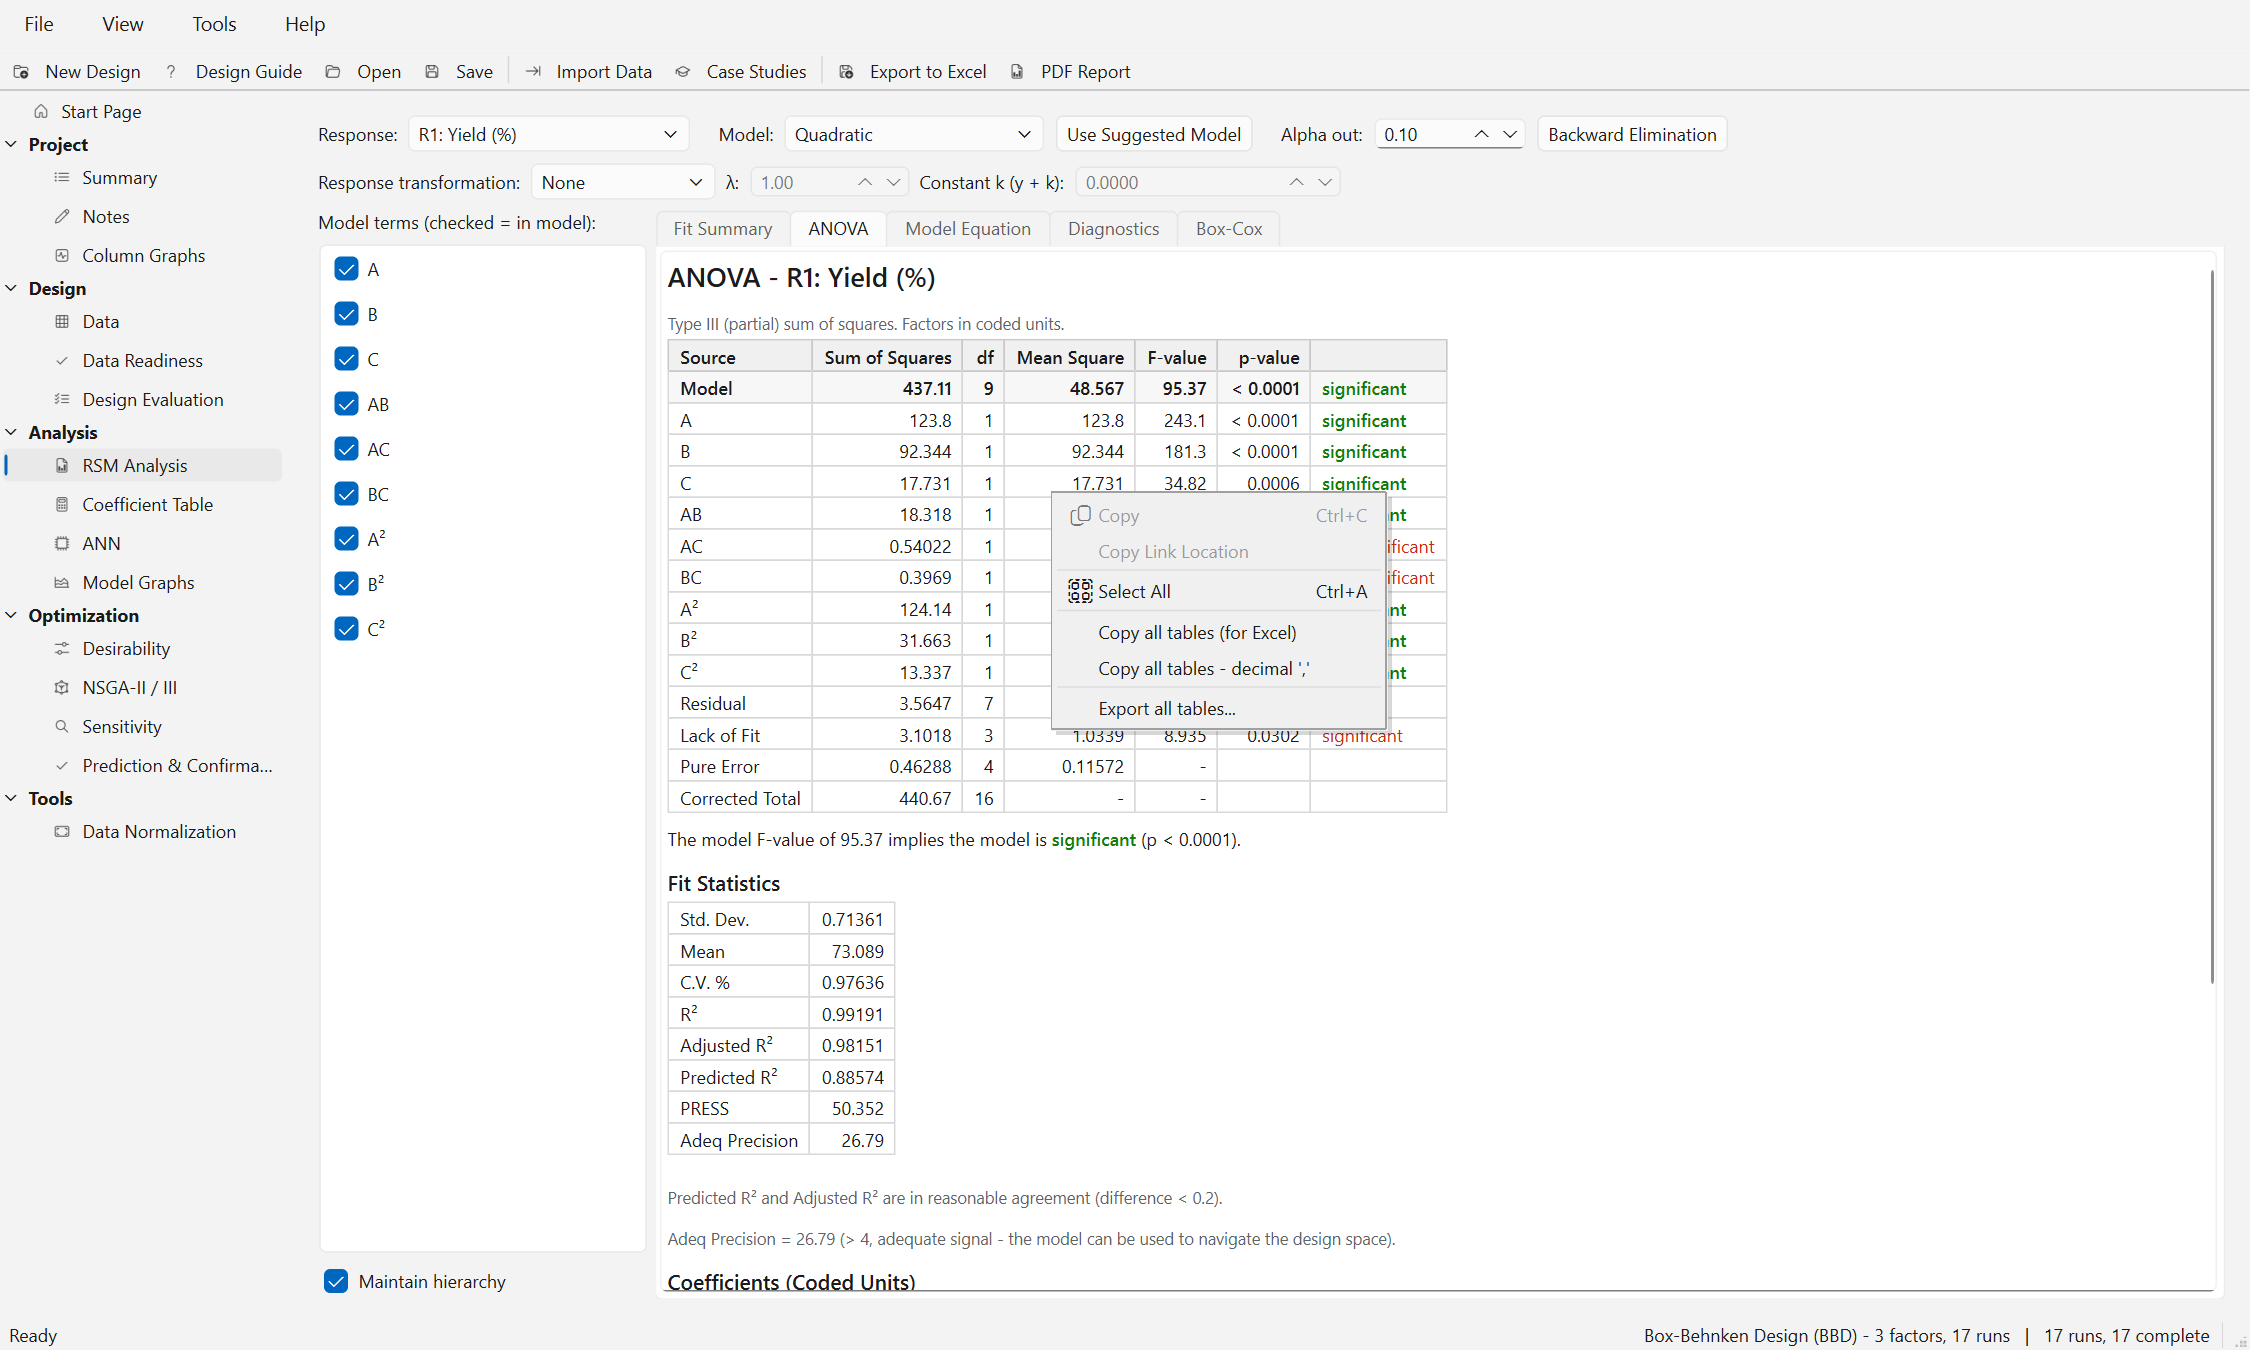
\includegraphics[width=0.5\linewidth]{report_context_menu.png}
\caption{Right-click menu of a report panel (RSM Analysis, ANOVA).}
\label{fig:ch02-reportmenu}
\end{figure}

\paragraph{Other exports.} The Data Normalization page has \ui{Export to Excel\dots} for the normalized data and
the normalization parameters, and the NSGA-II / III page has \ui{Export Pareto to Excel\dots} for the Pareto
solutions, the settings, the convergence history and the ANN vs RSM comparison (Chapter~\ref{chap:8}).

\section{Using several CPU cores}
\label{sec:ch02-cores}

ANN training, the automatic architecture search and the learning curve can run on several CPU cores. The number of
cores is set on the ANN page with \ui{CPU cores (parallel):} (shown as ``$n$ of $N$''); the default is all logical
cores minus one, so the computer stays responsive. Restarts, cross-validation folds and candidate architectures are
then computed at the same time in separate worker processes. The results are identical to those obtained with one
core, only faster; reduce the number if the computer is busy with other heavy programs or memory is short. The
worker processes are started on first use and closed automatically after 90 seconds without work.

The other computations (RSM, desirability, NSGA-II/III, sensitivity) run on one core. Long calculations run in the
background with a progress bar and a \ui{Stop} button, so the window stays responsive.

\section{A first session}
\label{sec:ch02-first}

\begin{figure}[htbp]
\centering
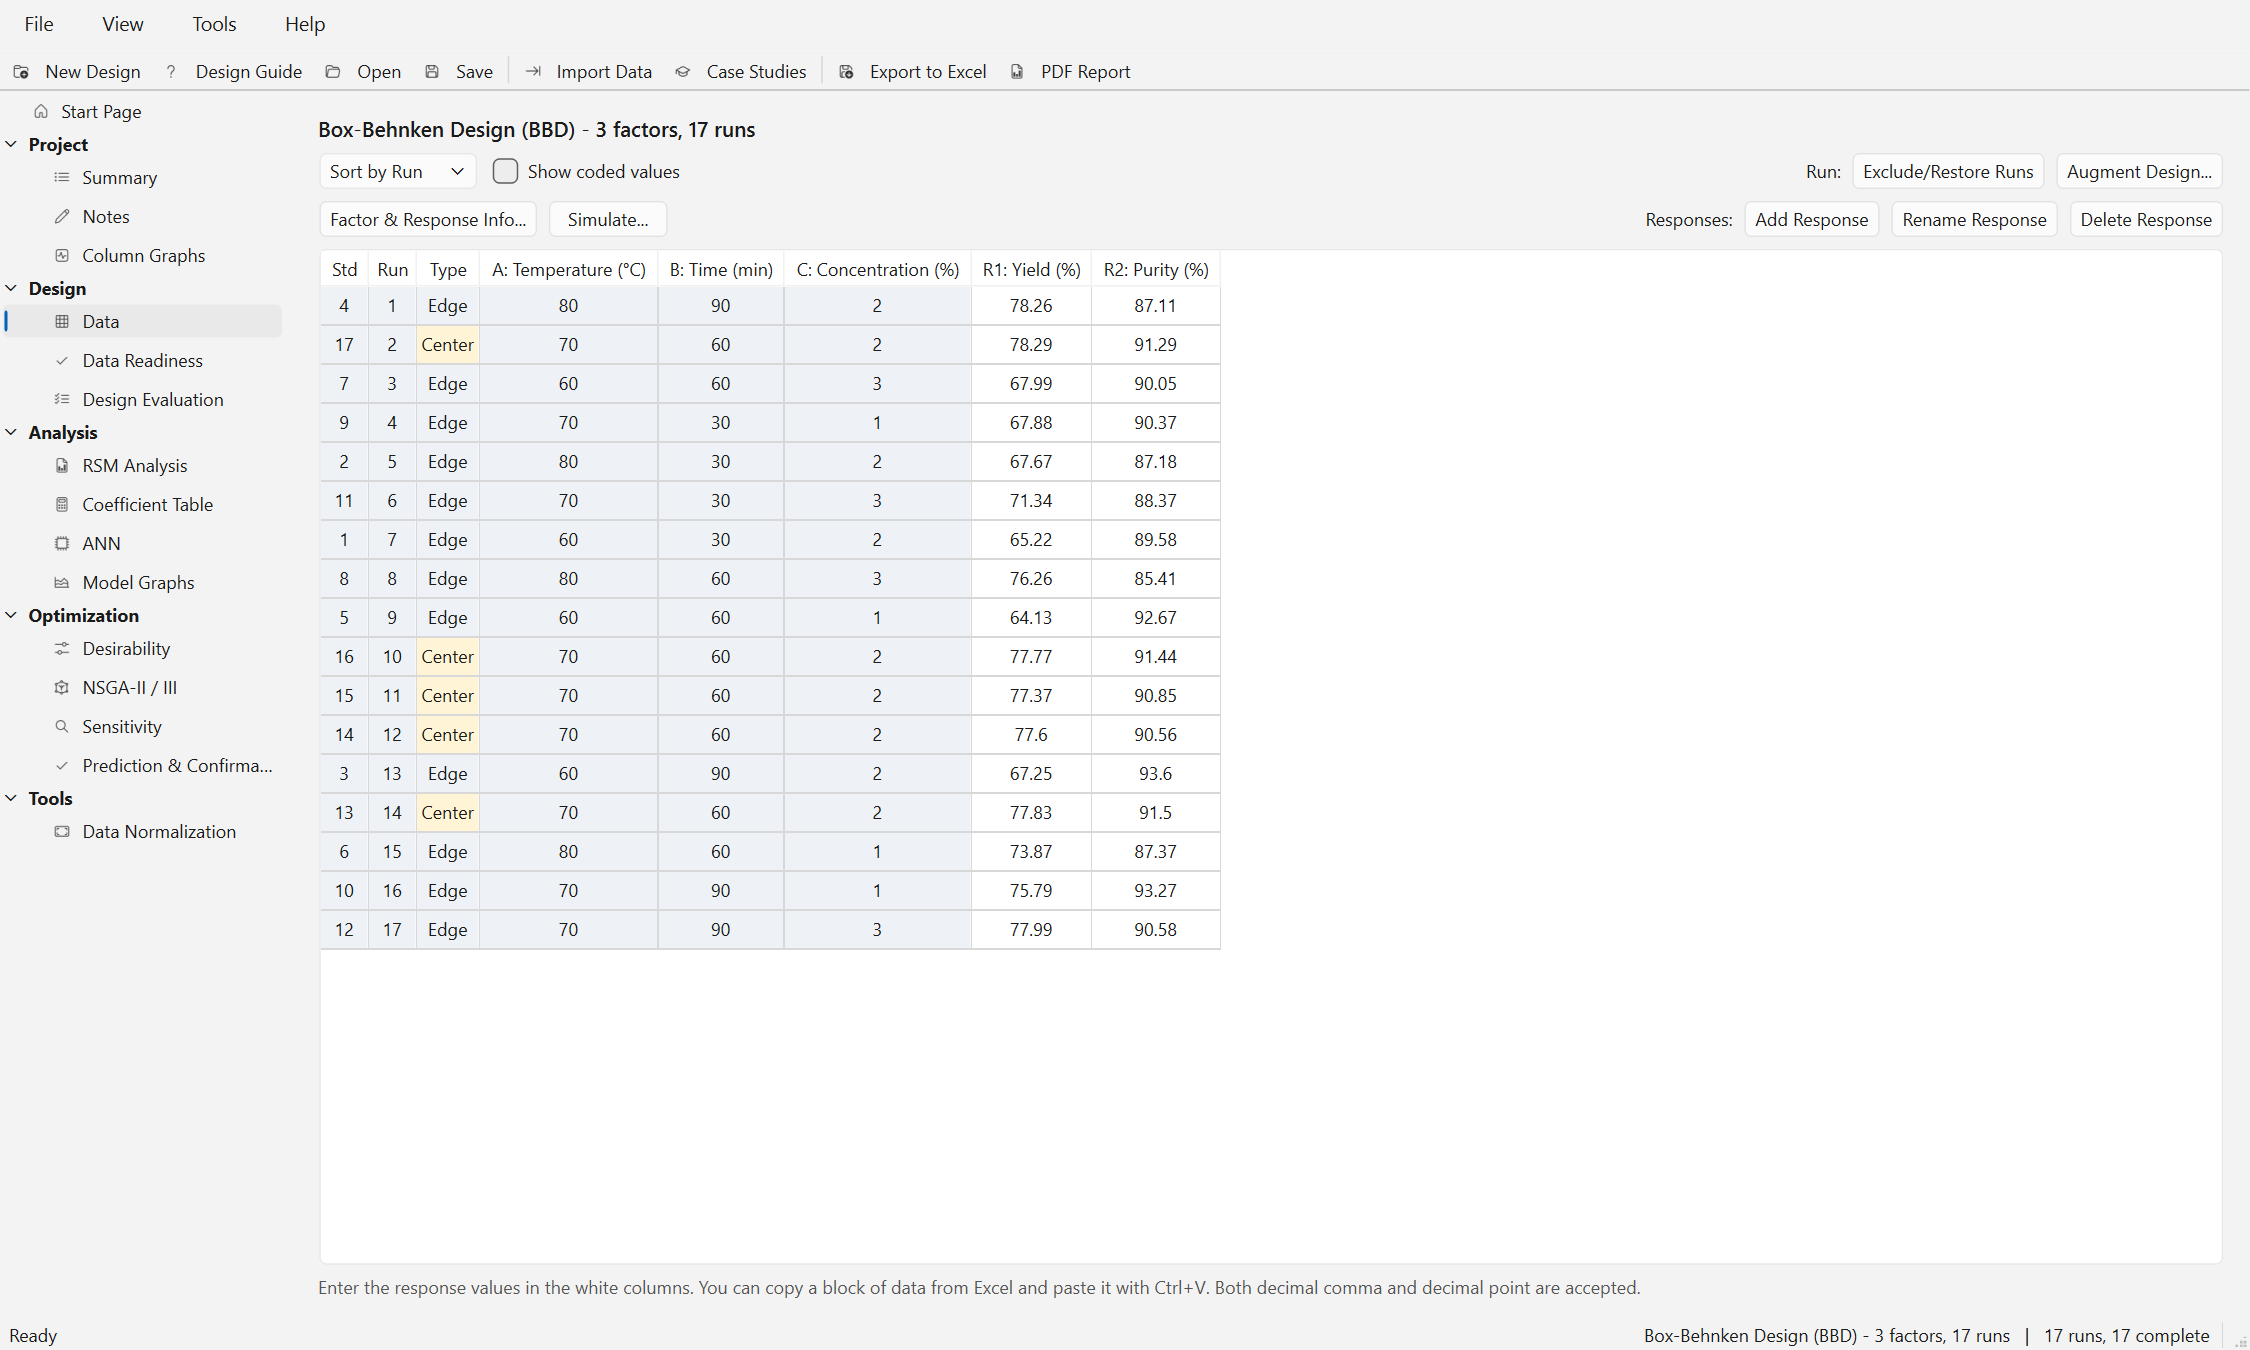
\includegraphics[width=0.8\linewidth]{data_page.png}
\caption{The Data page of the Box-Behnken extraction case study. Grey columns are factor settings (read-only in a
designed experiment), white columns are responses. The status bar shows ``17 runs, 17 complete''.}
\label{fig:ch02-data}
\end{figure}

A short tour with the first case study shows the main pages:
\begin{enumerate}
  \item Click \ui{Case studies} on the Start Page, select \ui{Extraction Optimization (Box-Behnken)} and click
        \ui{Open Case Study}. The Data page shows the 17 runs (Figure~\ref{fig:ch02-data}).
  \item Click \ui{Data Readiness}: the modeling and optimization scores of Yield are 94 and 96 (``Ready'').
  \item Click \ui{RSM Analysis}: the Fit Summary suggests the quadratic model; the ANOVA tab shows
        $R^2 = 0.9919$ and predicted $R^2 = 0.8857$ for Yield.
  \item Click \ui{Model Graphs} and choose \ui{2D Contour} or \ui{3D Surface}.
  \item On \ui{Desirability}, set the goal of Yield and Purity to \ui{Maximize} and click \ui{Run Optimization};
        then click \ui{Send Selected Solution to Prediction}.
  \item Save the project with \menupath{File $\rightarrow$ Save} and create a report with
        \menupath{File $\rightarrow$ PDF Report\dots}.
\end{enumerate}
Chapter~\ref{chap:11} continues this example in full detail.
